\section{Idea}

Para la metaeuristica de GRASP, tomaremos el algorimto goloso previamente implementado y lo combinaremos con las diferentes busquedas locales tambien previamente implementadas.

La idea es la siguiente, para cada paso del algoritmo, corremos primero la heuristica golosa con un orden aleaotrio en sus nodos. Este orden aleatorio, como ya hemos demostrado en el apartado del algoritmo goloso, podrá ir produciendo diferentes respuestas, cada una con una mejor o peor aproximación a la respuesta exacta.

Luego a la solución obtenida por el algoritmo goloso se le aplicarán una o varias de las busquedas locales implementadas en un intento de aproximar mas aun la respuesta al optimo.

Como primer criterio de corte el algoritmo se correrá un numero finito de veces, que será determinado en el momento de experimentación.

Como segundo criterio de corte se realizarán estos mismos pasos hasta que luego de un numero $x$ a determinar de intentos no haya sido posible mejorar la solución. En este punto se entrega la mejor respuesta obtenida hasta el momento.

Tras realizar diversas experimentaciones nos quedamos con dos versiones de GRASP, una que en el paso de busqueda local usa la busqueda local 2, y otra que en el paso de busqueda local primero utiliza una busqueda local 1 y luego una busqueda local 3.

A continuación se formaliza de manera mas precisa el algoritmo:

\begin{algorithm}
  	\begin{algorithmic}[1]\parskip=1mm
		 \caption{ GRASP1(SoluciónInicial) }
		 \STATE{while(1)}
		 	\STATE{\quad Genero una solucion incial a partir del Algoritmo Goloso}
		 	\STATE{\quad Utilizo busqueda local 2 para mejorar la solución incial}
		 	\STATE{\quad Si conseguí una mejor solucion que antes, la guardo}
		 	\STATE{\quad Si tras 1000 iteraciones no se pudo consegir una mejor solución}
		 	\STATE{\quad\quad Devuelvo la solución}
	\end{algorithmic}
\end{algorithm}

\begin{algorithm}
  	\begin{algorithmic}[1]\parskip=1mm
		 \caption{ GRASP2(SoluciónInicial) }
		 \STATE{while(1)}
		 	\STATE{\quad Genero una solucion incial a partir del Algoritmo Goloso}
		 	\STATE{\quad Utilizo busqueda local 1 para mejorar la solución}
		 	\STATE{\quad Utilizo busqueda local 3 para mejorar la solución}
		 	\STATE{\quad Si conseguí una mejor solucion que antes, la guardo}
		 	\STATE{\quad Si tras 1000 iteraciones no se pudo consegir una mejor solución}
		 	\STATE{\quad\quad Devuelvo la mejor solución}
	\end{algorithmic}
\end{algorithm}

\section{Experimentación}

Ahora haremos una experimentacion donde compararemos los tiempos de ejecución y los resultados del algoritmo de GRASP contra la solución exacta obtenida por backtracking.

Primero tomamos grafos de $25$ a $100$ nodos completos con aristas uniformemente distribuidas de $1$ a $100$ y analizamos los tiempos que dan los algoritmos:

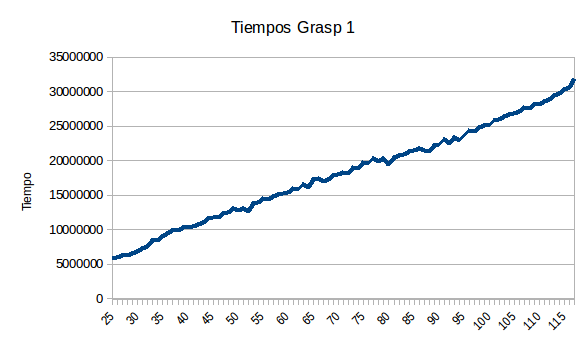
\includegraphics[scale=0.5]{Ej5/tiempog1.png}

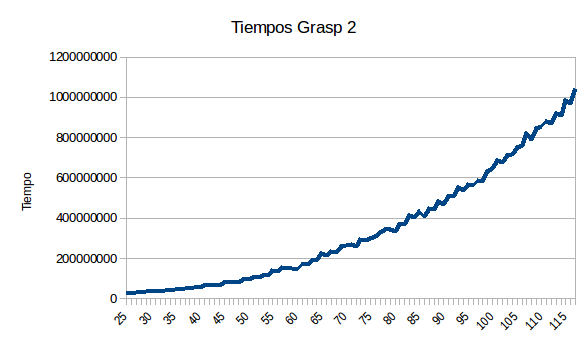
\includegraphics[scale=0.5]{Ej5/tiempog2.png}

Si bien se puede ver que no es exponencial, estas metaheuristicas dependen tanto de factores inheritos al algoritmo que se vuelve dificil de encontrar una complejidad de peor caso.

Ademas, se comparan como en los casos anteriores, las soluciones dadas por las dos heuristicas contra la solución exacta. La experimentacion para este caso es igual a la realizada para el algoritmo goloso y para las busquedas locales:

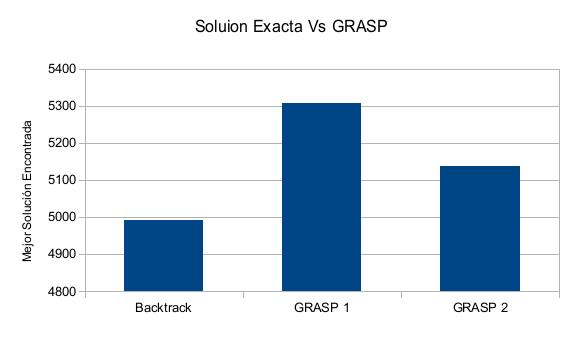
\includegraphics[scale=0.5]{Ej5/graspSol.jpg}

Puede verse aquí que la mejor de las heuristicas es la del GRASP 2, que no solo encuentra soluciones mas cercanas a la original, sinó que en 17 de los 100 casos, logra encontrar la solución exacta. Esto, seguramente debido a que usa la busqueda local 1, que como ya habíamos constatado en su experimentación, tambien lograba alcanzar soluciones exactas.

Finalmente, para los mismos casos de prueba antes vistos, tambien se miden los tiempos que tardan en encontrar la respuesta, obteniendose los siguientes resultados:

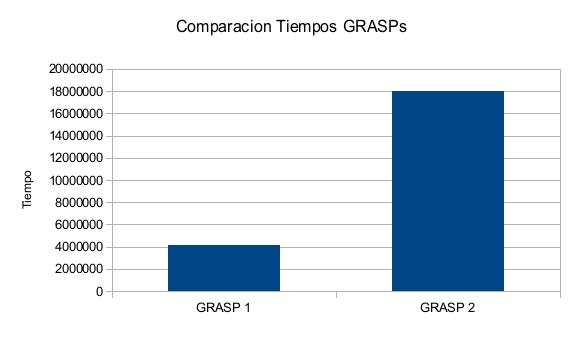
\includegraphics[scale=0.5]{Ej5/tiempos.jpg}

Puede verse que el hecho de encontrar soluciones exactas tiene su contrapartida en el hecho de que la metaheuristica tarde significativamente mas que la que no los encuentra.